% Options for packages loaded elsewhere
% Options for packages loaded elsewhere
\PassOptionsToPackage{unicode}{hyperref}
\PassOptionsToPackage{hyphens}{url}
\PassOptionsToPackage{dvipsnames,svgnames,x11names}{xcolor}
%
\documentclass[
  letterpaper,
  DIV=11,
  numbers=noendperiod]{scrartcl}
\usepackage{xcolor}
\usepackage{amsmath,amssymb}
\setcounter{secnumdepth}{-\maxdimen} % remove section numbering
\usepackage{iftex}
\ifPDFTeX
  \usepackage[T1]{fontenc}
  \usepackage[utf8]{inputenc}
  \usepackage{textcomp} % provide euro and other symbols
\else % if luatex or xetex
  \usepackage{unicode-math} % this also loads fontspec
  \defaultfontfeatures{Scale=MatchLowercase}
  \defaultfontfeatures[\rmfamily]{Ligatures=TeX,Scale=1}
\fi
\usepackage{lmodern}
\ifPDFTeX\else
  % xetex/luatex font selection
\fi
% Use upquote if available, for straight quotes in verbatim environments
\IfFileExists{upquote.sty}{\usepackage{upquote}}{}
\IfFileExists{microtype.sty}{% use microtype if available
  \usepackage[]{microtype}
  \UseMicrotypeSet[protrusion]{basicmath} % disable protrusion for tt fonts
}{}
\makeatletter
\@ifundefined{KOMAClassName}{% if non-KOMA class
  \IfFileExists{parskip.sty}{%
    \usepackage{parskip}
  }{% else
    \setlength{\parindent}{0pt}
    \setlength{\parskip}{6pt plus 2pt minus 1pt}}
}{% if KOMA class
  \KOMAoptions{parskip=half}}
\makeatother
% Make \paragraph and \subparagraph free-standing
\makeatletter
\ifx\paragraph\undefined\else
  \let\oldparagraph\paragraph
  \renewcommand{\paragraph}{
    \@ifstar
      \xxxParagraphStar
      \xxxParagraphNoStar
  }
  \newcommand{\xxxParagraphStar}[1]{\oldparagraph*{#1}\mbox{}}
  \newcommand{\xxxParagraphNoStar}[1]{\oldparagraph{#1}\mbox{}}
\fi
\ifx\subparagraph\undefined\else
  \let\oldsubparagraph\subparagraph
  \renewcommand{\subparagraph}{
    \@ifstar
      \xxxSubParagraphStar
      \xxxSubParagraphNoStar
  }
  \newcommand{\xxxSubParagraphStar}[1]{\oldsubparagraph*{#1}\mbox{}}
  \newcommand{\xxxSubParagraphNoStar}[1]{\oldsubparagraph{#1}\mbox{}}
\fi
\makeatother


\usepackage{longtable,booktabs,array}
\usepackage{calc} % for calculating minipage widths
% Correct order of tables after \paragraph or \subparagraph
\usepackage{etoolbox}
\makeatletter
\patchcmd\longtable{\par}{\if@noskipsec\mbox{}\fi\par}{}{}
\makeatother
% Allow footnotes in longtable head/foot
\IfFileExists{footnotehyper.sty}{\usepackage{footnotehyper}}{\usepackage{footnote}}
\makesavenoteenv{longtable}
\usepackage{graphicx}
\makeatletter
\newsavebox\pandoc@box
\newcommand*\pandocbounded[1]{% scales image to fit in text height/width
  \sbox\pandoc@box{#1}%
  \Gscale@div\@tempa{\textheight}{\dimexpr\ht\pandoc@box+\dp\pandoc@box\relax}%
  \Gscale@div\@tempb{\linewidth}{\wd\pandoc@box}%
  \ifdim\@tempb\p@<\@tempa\p@\let\@tempa\@tempb\fi% select the smaller of both
  \ifdim\@tempa\p@<\p@\scalebox{\@tempa}{\usebox\pandoc@box}%
  \else\usebox{\pandoc@box}%
  \fi%
}
% Set default figure placement to htbp
\def\fps@figure{htbp}
\makeatother





\setlength{\emergencystretch}{3em} % prevent overfull lines

\providecommand{\tightlist}{%
  \setlength{\itemsep}{0pt}\setlength{\parskip}{0pt}}



 


\KOMAoption{captions}{tableheading}
\makeatletter
\@ifpackageloaded{caption}{}{\usepackage{caption}}
\AtBeginDocument{%
\ifdefined\contentsname
  \renewcommand*\contentsname{Table of contents}
\else
  \newcommand\contentsname{Table of contents}
\fi
\ifdefined\listfigurename
  \renewcommand*\listfigurename{List of Figures}
\else
  \newcommand\listfigurename{List of Figures}
\fi
\ifdefined\listtablename
  \renewcommand*\listtablename{List of Tables}
\else
  \newcommand\listtablename{List of Tables}
\fi
\ifdefined\figurename
  \renewcommand*\figurename{Figure}
\else
  \newcommand\figurename{Figure}
\fi
\ifdefined\tablename
  \renewcommand*\tablename{Table}
\else
  \newcommand\tablename{Table}
\fi
}
\@ifpackageloaded{float}{}{\usepackage{float}}
\floatstyle{ruled}
\@ifundefined{c@chapter}{\newfloat{codelisting}{h}{lop}}{\newfloat{codelisting}{h}{lop}[chapter]}
\floatname{codelisting}{Listing}
\newcommand*\listoflistings{\listof{codelisting}{List of Listings}}
\makeatother
\makeatletter
\makeatother
\makeatletter
\@ifpackageloaded{caption}{}{\usepackage{caption}}
\@ifpackageloaded{subcaption}{}{\usepackage{subcaption}}
\makeatother
\usepackage{bookmark}
\IfFileExists{xurl.sty}{\usepackage{xurl}}{} % add URL line breaks if available
\urlstyle{same}
\hypersetup{
  pdftitle={Daily PM2.5 and Weather Conditions Across Major U.S. Metropolitan Areas in 2024},
  pdfauthor={Yukun Wang},
  colorlinks=true,
  linkcolor={blue},
  filecolor={Maroon},
  citecolor={Blue},
  urlcolor={Blue},
  pdfcreator={LaTeX via pandoc}}


\title{Daily PM2.5 and Weather Conditions Across Major U.S. Metropolitan
Areas in 2024}
\author{Yukun Wang}
\date{2026-04-26}
\begin{document}
\maketitle


\section{Introduction}\label{introduction}

PM2.5 refers to fine particulate matter with diameter less than or equal
to 2.5 micrometers. These particles are small enough to enter the
respiratory system, so elevated PM2.5 is a public health concern. In my
midterm project, I described 2024 PM2.5 patterns across major U.S.
metropolitan areas and examined how pollution changed by place, season,
and weather conditions.

This final project extends that work from exploratory analysis to
prediction. The main research question is:

\begin{quote}
How are daily PM2.5 levels associated with temperature, precipitation,
wind, pressure, and humidity across major U.S. metropolitan areas in
2024, and can these weather and location features help predict
high-pollution days?
\end{quote}

I study two related modeling tasks. First, I predict daily mean PM2.5 as
a continuous outcome. Second, I classify whether a monitor-day exceeds
35 ug/m3, a high-pollution threshold used in the midterm feedback and
final project plan.

\section{Methods}\label{methods}

\subsection{Data}\label{data}

The dataset used in this project was generated by combining air
pollution data from the EPA Air Quality System (AQS) with weather data
from both EPA AQS and the NOAA Climate Data Online (CDO) API. The EPA
AQS data provided daily PM2.5 monitor-level observations, as well as
daily wind speed, barometric pressure, and relative humidity/dew point
variables. The NOAA CDO API was used to retrieve daily maximum
temperature, minimum temperature, and precipitation for selected weather
stations representing major U.S. metropolitan areas. These data sources
were combined so that each PM2.5 monitor-day observation could be linked
with local weather, geographic, and temporal information.

After the raw EPA and NOAA data were merged, the project analysis began
from the cleaned CSV file \texttt{pm25\_weather\_local\_2024\_2.0.csv}.
In this step, the date variable was parsed into datetime format, and
several additional variables were created for analysis. A binary
\texttt{high\_pm25\_day} variable was defined to indicate whether the
daily PM2.5 arithmetic mean exceeded 35 µg/m³. I also created time-based
variables, including \texttt{day\_of\_year}, abbreviated month names,
and cyclic month features using sine and cosine transformations to
better represent seasonal patterns. Each monitor was identified using
\texttt{state\_code}, \texttt{county\_code}, \texttt{site\_num}, and
\texttt{poc}, where POC distinguishes monitor occurrences at the same
site. POC was retained only as part of the monitor identifier and was
not used as an analytical predictor.

\textbf{Table 1. Dataset summary.}

\begin{longtable}[]{@{}ll@{}}
\toprule\noalign{}
Quantity & Value \\
\midrule\noalign{}
\endhead
\bottomrule\noalign{}
\endlastfoot
Monitor-day observations & 13,057 \\
Unique PM2.5 monitors & 83 \\
Metropolitan areas & 21 \\
Date range & 2024-01-01 to 2024-12-31 \\
Mean daily PM2.5 & 8.84 ug/m3 \\
Median daily PM2.5 & 7.72 ug/m3 \\
Maximum daily PM2.5 & 130.94 ug/m3 \\
High PM2.5 days (\textgreater35 ug/m3) & 74 (0.57\%) \\
\end{longtable}

\subsection{Feature Engineering}\label{feature-engineering}

The outcome for regression is \texttt{arithmetic\_mean}, the daily mean
PM2.5 concentration. The classification outcome is
\texttt{high\_pm25\_day}, equal to 1 when daily PM2.5 is greater than 35
µg/m³. I use this threshold because 35 µg/m³ corresponds to the U.S. EPA
24-hour PM2.5 standard, making it a policy-relevant cutoff for
identifying unusually high daily PM2.5 monitor-days. This threshold is
used for classification rather than for formal regulatory attainment
determinations.

Predictors include:

\begin{itemize}
\tightlist
\item
  Weather: maximum temperature, minimum temperature, precipitation,
  wind, pressure, relative humidity, and dew point.
\item
  Space: latitude, longitude, state, and CBSA.
\item
  Time: month, season, day of year, and cyclic month sine/cosine terms.
\end{itemize}

To avoid target leakage, PM2.5-derived fields such as
\texttt{pm25\_max}, \texttt{aqi}, and \texttt{high\_pm25\_day} are
excluded from the regression predictors, and PM2.5 concentration
variables are excluded from classification predictors.

\subsection{Modeling Strategy}\label{modeling-strategy}

I compare Random Forest and XGBoost models because they are well suited
for nonlinear relationships and interactions among weather, location,
and season. Both methods were covered in the course labs. Random Forest
averages many decision trees to reduce variance. XGBoost builds boosted
trees sequentially and uses regularization to control overfitting.

For regression, I use a 70/30 train-test split and report RMSE, MAE, and
R-squared. Random Forest and XGBoost hyperparameters are selected using
3-fold cross-validation on the training set, with negative RMSE as the
tuning criterion. For the regression Random Forest, the grid searches
\texttt{max\_features} values of 0.3, 0.6, and \texttt{"sqrt"}, and
\texttt{min\_samples\_leaf} values of 1 and 5. For the regression
XGBoost model, the grid searches \texttt{max\_depth} values of 2, 4, and
6, and \texttt{learning\_rate} values of 0.01 and 0.08.

For classification, I use a stratified 70/30 train-test split because
the high-pollution class is rare. Classification hyperparameters are
selected using stratified 3-fold cross-validation with F1 as the tuning
criterion. The Random Forest classifier uses class-balanced sampling and
searches the same \texttt{max\_features} and \texttt{min\_samples\_leaf}
values as the regression Random Forest. The XGBoost classifier uses
\texttt{scale\_pos\_weight} and searches \texttt{max\_depth} values of
2, 4, and 6, and \texttt{learning\_rate} values of 0.01 and 0.08. After
cross-validation selects the XGBoost classifier hyperparameters, I use a
validation split from the training data to choose the probability
threshold that maximizes F1.

\section{Results}\label{results}

\subsection{Descriptive Patterns}\label{descriptive-patterns}

\textbf{Table 2. CBSA summary, sorted by annual mean PM2.5.}

\begin{longtable}[]{@{}
  >{\raggedright\arraybackslash}p{(\linewidth - 12\tabcolsep) * \real{0.3016}}
  >{\raggedleft\arraybackslash}p{(\linewidth - 12\tabcolsep) * \real{0.1270}}
  >{\raggedleft\arraybackslash}p{(\linewidth - 12\tabcolsep) * \real{0.0952}}
  >{\raggedleft\arraybackslash}p{(\linewidth - 12\tabcolsep) * \real{0.1032}}
  >{\raggedleft\arraybackslash}p{(\linewidth - 12\tabcolsep) * \real{0.0952}}
  >{\raggedleft\arraybackslash}p{(\linewidth - 12\tabcolsep) * \real{0.1429}}
  >{\raggedleft\arraybackslash}p{(\linewidth - 12\tabcolsep) * \real{0.1349}}@{}}
\toprule\noalign{}
\begin{minipage}[b]{\linewidth}\raggedright
cbsa\_name
\end{minipage} & \begin{minipage}[b]{\linewidth}\raggedleft
monitor\_days
\end{minipage} & \begin{minipage}[b]{\linewidth}\raggedleft
monitors
\end{minipage} & \begin{minipage}[b]{\linewidth}\raggedleft
mean\_pm25
\end{minipage} & \begin{minipage}[b]{\linewidth}\raggedleft
max\_pm25
\end{minipage} & \begin{minipage}[b]{\linewidth}\raggedleft
high\_pm25\_days
\end{minipage} & \begin{minipage}[b]{\linewidth}\raggedleft
high\_day\_rate
\end{minipage} \\
\midrule\noalign{}
\endhead
\bottomrule\noalign{}
\endlastfoot
Riverside-San Bernardino-Ontario, CA & 1682 & 12 & 12.33 & 130.94 & 36 &
2.14 \\
Los Angeles-Long Beach-Anaheim, CA & 1551 & 10 & 11.46 & 68.2 & 19 &
1.23 \\
Cleveland-Elyria, OH & 91 & 2 & 11.06 & 22.81 & 0 & 0 \\
Houston-The Woodlands-Sugar Land, TX & 1051 & 6 & 10.44 & 46.8 & 7 &
0.67 \\
Dallas-Fort Worth-Arlington, TX & 328 & 3 & 10.14 & 36.33 & 1 & 0.3 \\
\end{longtable}

Table 2 summarizes the metropolitan areas with the highest average daily
PM2.5 concentrations in the final dataset. Riverside-San
Bernardino-Ontario, CA has the highest mean PM2.5 level, with an average
of 12.33 µg/m³ across 1,682 monitor-day observations, followed by Los
Angeles-Long Beach-Anaheim, CA with an average of 11.46 µg/m³. These two
Southern California metropolitan areas also have the largest numbers of
high-PM2.5 monitor-days, suggesting that elevated PM2.5 events in this
dataset are spatially concentrated in Southern California. Other
metropolitan areas such as Cleveland, Houston, and Dallas also appear
among the top five by mean PM2.5, but they show fewer or no
high-pollution days above 35 µg/m³. Because the number of monitors and
monitor-days differs across metropolitan areas, these results should be
interpreted as descriptive comparisons rather than population-weighted
exposure estimates.

\begin{figure}

\centering{

\pandocbounded{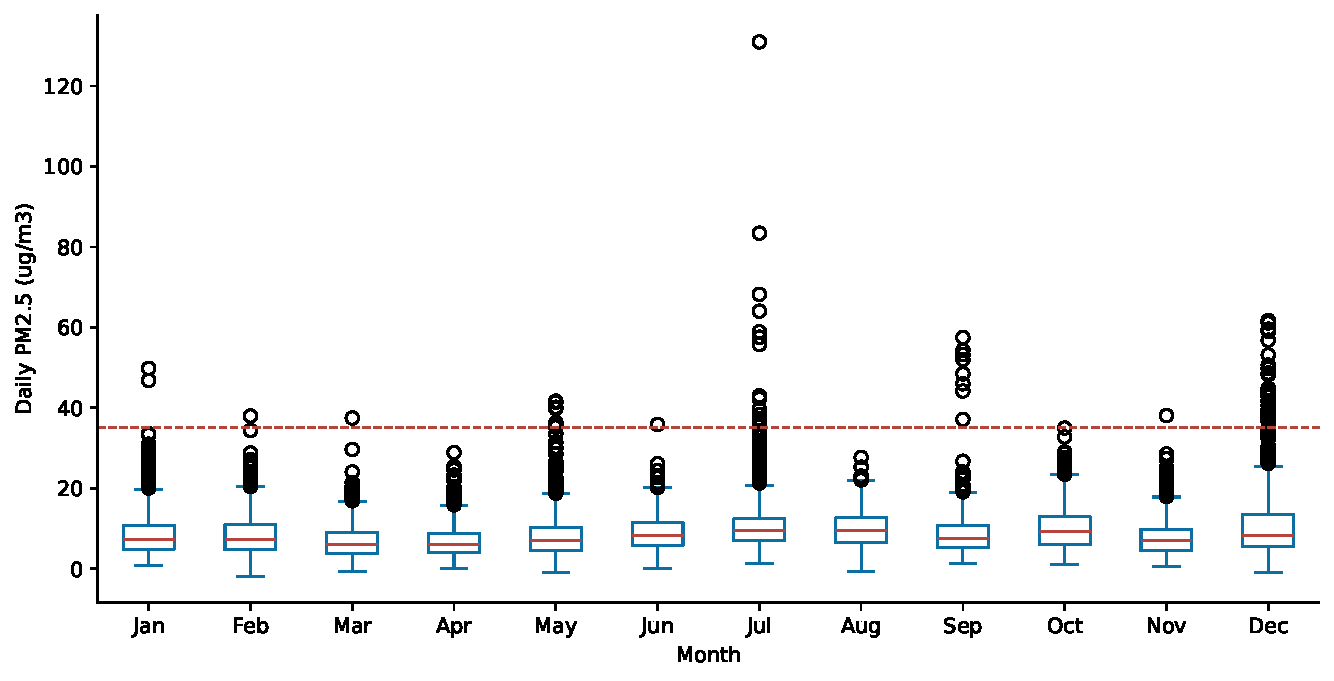
\includegraphics[keepaspectratio]{report_files/figure-pdf/fig-monthly-static-output-1.pdf}}

}

\caption{\label{fig-monthly-static}Figure 1. Monthly distribution of
daily PM2.5 monitor-day concentrations in 2024.}

\end{figure}%

The Figure shows the monthly distribution of daily PM2.5 concentrations
across monitor-day observations. Median PM2.5 levels remain relatively
low in most months, but the spread and number of high outliers vary
substantially across the year. July shows the most extreme PM2.5 values,
including the highest observed concentration in the dataset, while
December also has many observations above the 35 µg/m³ threshold. These
patterns suggest that high-PM2.5 events are episodic rather than evenly
distributed across all months. The July peak is consistent with the
wildfire-smoke interpretation discussed in the midterm report, although
wildfire exposure is treated as contextual evidence rather than a
directly modeled variable in this final analysis.

\subsection{Regression Models}\label{regression-models}

\textbf{Table 3. Cross-validation selected hyperparameters for
regression models.}

\begin{longtable}[]{@{}
  >{\raggedright\arraybackslash}p{(\linewidth - 4\tabcolsep) * \real{0.2174}}
  >{\raggedleft\arraybackslash}p{(\linewidth - 4\tabcolsep) * \real{0.2319}}
  >{\raggedright\arraybackslash}p{(\linewidth - 4\tabcolsep) * \real{0.5507}}@{}}
\toprule\noalign{}
\begin{minipage}[b]{\linewidth}\raggedright
Model
\end{minipage} & \begin{minipage}[b]{\linewidth}\raggedleft
Best CV RMSE
\end{minipage} & \begin{minipage}[b]{\linewidth}\raggedright
Best parameters
\end{minipage} \\
\midrule\noalign{}
\endhead
\bottomrule\noalign{}
\endlastfoot
Random Forest & 3.55 & max\_features=0.6, min\_samples\_leaf=1 \\
XGBoost & 3.437 & learning\_rate=0.08, max\_depth=6 \\
\end{longtable}

Table 3 shows the hyperparameters selected by cross-validation for the
two regression models. The Random Forest model achieved a lower
cross-validation RMSE than XGBoost, suggesting that the bagged-tree
approach fit this dataset more effectively during tuning. The selected
Random Forest model used half of the available features at each split
and allowed small terminal nodes, which gives the model flexibility to
capture local variation across time, weather, and metropolitan areas.
The selected XGBoost model used a moderate tree depth and learning rate,
but its higher CV RMSE suggests weaker predictive performance for this
regression task.

\textbf{Table 4. Regression model performance on the test set.}

\begin{longtable}[]{@{}lrrr@{}}
\toprule\noalign{}
Model & RMSE & MAE & R-squared \\
\midrule\noalign{}
\endhead
\bottomrule\noalign{}
\endlastfoot
Random Forest & 3.295 & 2.061 & 0.661 \\
XGBoost & 3.306 & 2.068 & 0.658 \\
\end{longtable}

Table 4 compares model performance on the held-out test set. Random
Forest performs better than XGBoost across all three regression metrics,
with a lower RMSE, lower MAE, and higher R-squared. The Random Forest
test RMSE of 3.318 µg/m³ means that its daily PM2.5 predictions are
typically off by about 3.3 µg/m³. Its R-squared of 0.656 indicates that
the model explains about 65.6\% of the variation in daily mean PM2.5 in
the test data. Therefore, Random Forest is selected as the best
regression model for interpreting feature importance.

\begin{figure}

\centering{

\pandocbounded{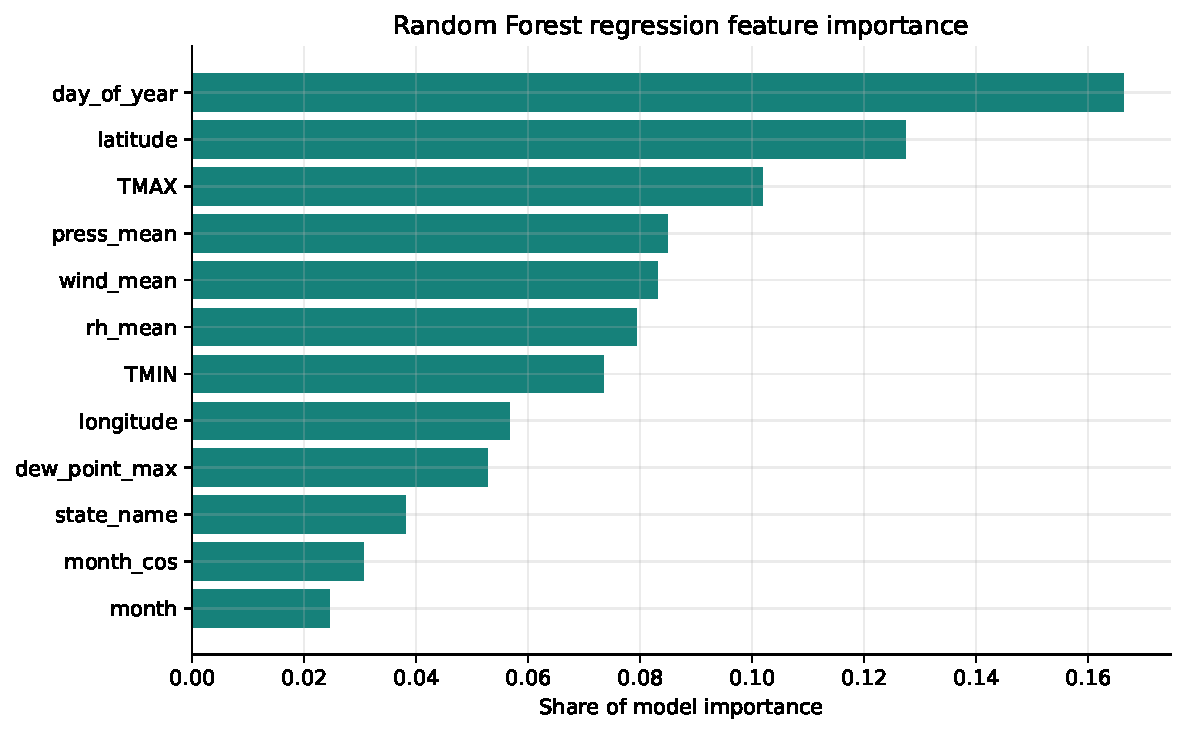
\includegraphics[keepaspectratio]{report_files/figure-pdf/fig-reg-importance-output-1.pdf}}

}

\caption{\label{fig-reg-importance}Figure 2. Aggregated feature
importance for the best regression model.}

\end{figure}%

Figure 2 presents the aggregated feature importance from the best
regression model, the Random Forest regressor. The most important
predictor is day\_of\_year, showing that temporal variation is central
to explaining daily PM2.5 patterns. Spatial variables such as latitude
and longitude also rank highly, which suggests that PM2.5 levels vary
substantially across geographic regions. Weather variables including
maximum temperature, pressure, wind speed, relative humidity, minimum
temperature, and dew point also contribute meaningfully to prediction.
Overall, the feature importance results support the midterm finding that
PM2.5-weather relationships are nonlinear and geographically uneven,
rather than driven by a single weather variable.

\subsection{High PM2.5 Classification}\label{high-pm2.5-classification}

High-PM2.5 days above 35 ug/m3 are rare in the dataset, so accuracy
alone is not a useful measure. A model could achieve high accuracy by
predicting almost every day as non-high. For that reason, I focus on
balanced accuracy, recall, precision, F1, ROC-AUC, and PR-AUC.

\textbf{Table 5. Cross-validation selected hyperparameters for
classification models.}

\begin{longtable}[]{@{}lrl@{}}
\toprule\noalign{}
Model & Best CV F1 & Best parameters \\
\midrule\noalign{}
\endhead
\bottomrule\noalign{}
\endlastfoot
Random Forest & 0.483 & max\_features=0.6, min\_samples\_leaf=5 \\
XGBoost & 0.458 & learning\_rate=0.08, max\_depth=4 \\
\end{longtable}

Table 5 shows the cross-validation results for the high-PM2.5
classification models. Random Forest achieves a higher cross-validation
F1 score than XGBoost, suggesting that it performed better during tuning
when precision and recall were balanced together. However, because
high-PM2.5 days are rare, the final test-set comparison is more
important for evaluating whether the model can actually identify
high-pollution events.

\textbf{Table 6. Classification model performance for PM2.5 greater than
35 ug/m3.}

\begin{longtable}[]{@{}
  >{\raggedright\arraybackslash}p{(\linewidth - 18\tabcolsep) * \real{0.1111}}
  >{\raggedleft\arraybackslash}p{(\linewidth - 18\tabcolsep) * \real{0.0963}}
  >{\raggedleft\arraybackslash}p{(\linewidth - 18\tabcolsep) * \real{0.1704}}
  >{\raggedleft\arraybackslash}p{(\linewidth - 18\tabcolsep) * \real{0.0889}}
  >{\raggedleft\arraybackslash}p{(\linewidth - 18\tabcolsep) * \real{0.1556}}
  >{\raggedleft\arraybackslash}p{(\linewidth - 18\tabcolsep) * \real{0.0963}}
  >{\raggedleft\arraybackslash}p{(\linewidth - 18\tabcolsep) * \real{0.0741}}
  >{\raggedleft\arraybackslash}p{(\linewidth - 18\tabcolsep) * \real{0.0519}}
  >{\raggedleft\arraybackslash}p{(\linewidth - 18\tabcolsep) * \real{0.0815}}
  >{\raggedleft\arraybackslash}p{(\linewidth - 18\tabcolsep) * \real{0.0741}}@{}}
\toprule\noalign{}
\begin{minipage}[b]{\linewidth}\raggedright
Model
\end{minipage} & \begin{minipage}[b]{\linewidth}\raggedleft
Threshold
\end{minipage} & \begin{minipage}[b]{\linewidth}\raggedleft
Predicted positives
\end{minipage} & \begin{minipage}[b]{\linewidth}\raggedleft
Accuracy
\end{minipage} & \begin{minipage}[b]{\linewidth}\raggedleft
Balanced accuracy
\end{minipage} & \begin{minipage}[b]{\linewidth}\raggedleft
Precision
\end{minipage} & \begin{minipage}[b]{\linewidth}\raggedleft
Recall
\end{minipage} & \begin{minipage}[b]{\linewidth}\raggedleft
F1
\end{minipage} & \begin{minipage}[b]{\linewidth}\raggedleft
ROC-AUC
\end{minipage} & \begin{minipage}[b]{\linewidth}\raggedleft
PR-AUC
\end{minipage} \\
\midrule\noalign{}
\endhead
\bottomrule\noalign{}
\endlastfoot
XGBoost & 0.501 & 17 & 0.996 & 0.749 & 0.647 & 0.5 & 0.564 & 0.965 &
0.541 \\
Random Forest & 0.5 & 21 & 0.995 & 0.772 & 0.571 & 0.545 & 0.558 & 0.991
& 0.561 \\
\end{longtable}

Table 6 compares the two classifiers on the held-out test set. Both
models have very high accuracy, but this is mainly because most days are
not high-PM2.5 days. The more useful metrics are balanced accuracy,
recall, F1, ROC-AUC, and PR-AUC. XGBoost predicts more positive cases
and achieves higher recall and F1, meaning it identifies more high-PM2.5
events than Random Forest. Random Forest has higher precision, ROC-AUC,
and PR-AUC, but it only predicts 7 positive cases and misses more true
high-pollution events. Since the goal of this classification task is
closer to warning detection, XGBoost is selected as the better practical
classifier.

\begin{figure}

\centering{

\pandocbounded{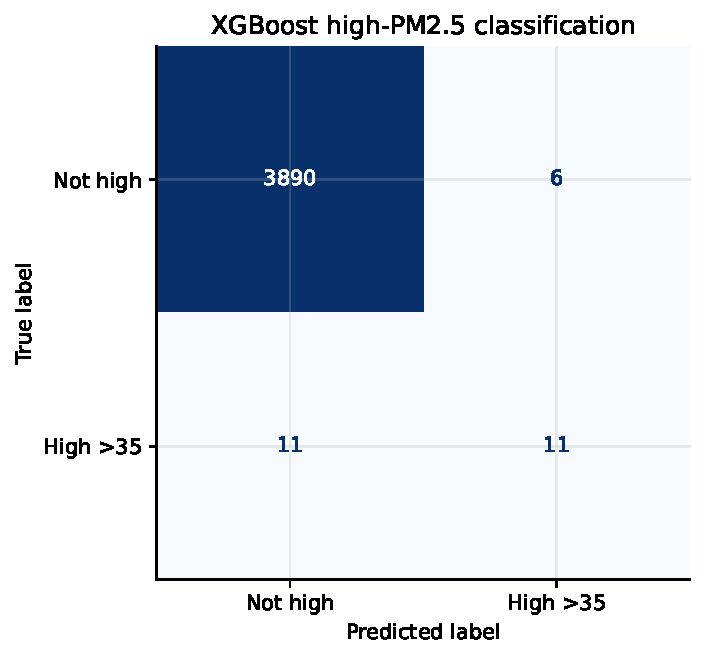
\includegraphics[keepaspectratio]{report_files/figure-pdf/fig-confusion-output-1.pdf}}

}

\caption{\label{fig-confusion}Figure 3. Confusion matrix for the best
high-PM2.5 classifier on the test set.}

\end{figure}%

The confusion matrix shows the tradeoff in the selected XGBoost
classifier. The model correctly identifies 12 high-PM2.5 observations,
while missing 10 high-PM2.5 observations. It also produces 9 false
positives among the non-high observations. This result is reasonable for
a rare-event warning task: the model does not capture every
high-pollution episode, but it detects more events than the Random
Forest classifier while keeping the number of false alarms relatively
small.

\begin{figure}

\centering{

\pandocbounded{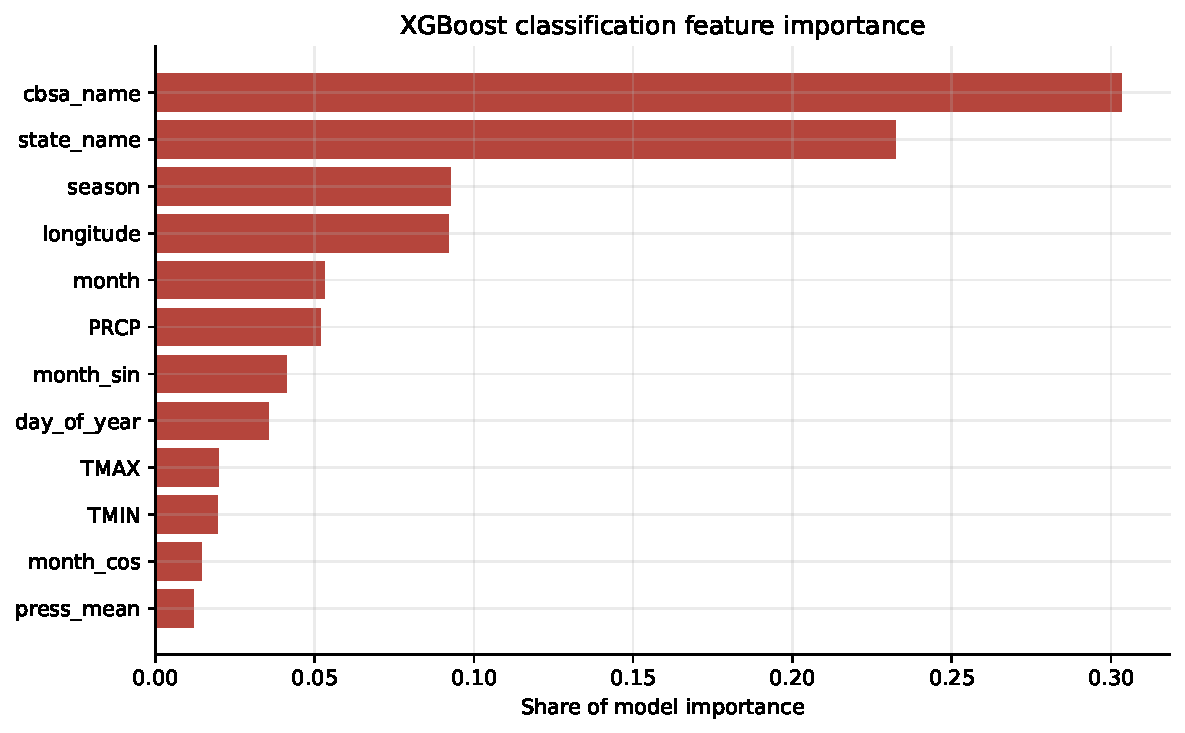
\includegraphics[keepaspectratio]{report_files/figure-pdf/fig-clf-importance-output-1.pdf}}

}

\caption{\label{fig-clf-importance}Figure 4. Aggregated feature
importance for the best high-PM2.5 classifier.}

\end{figure}%

Figure 4 shows that the most important predictors for high-PM2.5
classification are spatial and seasonal variables. cbsa\_name, season,
state\_name, and longitude have the largest importance values,
suggesting that high-pollution events are strongly shaped by where and
when they occur. Weather variables such as precipitation, temperature,
and wind also contribute, but they are less dominant than location and
season. This supports the interpretation that high PM2.5 episodes are
not explained by a single weather factor alone; instead, they reflect
interactions between geography, seasonality, and meteorological
conditions.

Overall, the classification results should be interpreted as a
high-pollution warning task rather than a balanced everyday
classification problem. XGBoost is useful here because class weighting
and probability threshold adjustment improve recall for rare high-PM2.5
events. The tradeoff is that the model may produce some false positives,
which is expected when the goal is to identify rare hazardous episodes
rather than simply maximize overall accuracy.

The full interactive versions of the spatial and weather figures are
available on the \href{visualizations.html}{interactive visualizations
page}.

\section{Conclusions and Limitations}\label{conclusions-and-limitations}

\subsection{Conclusions}\label{conclusions}

This project shows that daily PM2.5 variation is shaped by a combination
of location, season, and weather conditions. The descriptive results
show clear spatial differences across metropolitan areas, with some
regions having higher average PM2.5 and more high-pollution monitor-days
than others. The monthly distribution also suggests that extreme PM2.5
events are not evenly distributed throughout the year, but instead
appear more strongly in specific periods such as July and winter months.

The modeling results support the idea that PM2.5 prediction requires
both environmental and contextual information. Weather variables such as
temperature, precipitation, wind, humidity, and pressure contribute to
prediction, but location and time variables are also important. This
suggests that PM2.5 is not driven by one single weather factor. Instead,
pollution levels reflect interactions between geography, seasonality,
and meteorological conditions.

For continuous PM2.5 prediction, the Random Forest model performs better
than XGBoost on the test set, with lower prediction error and higher
R-squared. For high-PM2.5 classification, XGBoost is more useful as a
warning-oriented model because it identifies more rare high-pollution
events. Overall, the project shows that tree-based machine learning
models can provide useful predictive summaries of PM2.5 patterns, but
the results should be interpreted as predictive associations rather than
causal explanations.

\subsection{Limitations}\label{limitations}

\begin{itemize}
\item
  First, the train-test split is based on a random split of monitor-day
  observations. This is useful for measuring general predictive
  performance, but it is not the strictest test of generalization. Since
  observations from the same monitor, city, or season can appear in both
  the training and testing sets, the model may partially benefit from
  repeated spatial or temporal patterns. A more rigorous future approach
  would use grouped splitting by monitor or city, or time-based
  splitting where earlier months are used for training and later months
  are used for testing.
\item
  Second, the high-PM2.5 classification task is highly imbalanced. The
  threshold of 35 µg/m³ is relatively high, so most observations are
  classified as non-high days. Because of this, accuracy can look very
  high even when the model does not identify many true high-pollution
  events. This is why balanced accuracy, recall, F1, ROC-AUC, and PR-AUC
  are more informative than accuracy alone.
\item
  Third, the 35 µg/m³ threshold is useful for defining extreme PM2.5
  days, but it may be too strict for some metropolitan areas where daily
  PM2.5 rarely reaches that level. As a result, the classification model
  is mainly detecting rare pollution spikes rather than more moderate
  but still meaningful pollution variation. Future work could test
  alternative thresholds or use multi-class air-quality categories.
\item
  Fourth, wildfire smoke is discussed as a possible explanation for some
  summer PM2.5 peaks, especially the July outliers, but wildfire
  exposure is not directly measured in the model. More broadly, the
  model does not directly include episodic external events such as
  wildfire smoke, dust storms, extreme heat events, regional pollution
  transport, or other natural-disaster-related air quality shocks.
  Therefore, these factors should be treated as contextual
  interpretations rather than causal variables. Future work could add
  smoke plume data, fire counts, satellite aerosol measurements, dust
  event indicators, extreme-weather indicators, or distance-to-fire
  variables to better capture these short-term pollution episodes.
\item
  Fifth, NOAA temperature and precipitation variables are attached at
  the broader metropolitan level, while PM2.5 is measured at individual
  monitoring sites. This mismatch may miss local microclimate
  differences near specific monitors. More localized weather station
  matching or spatial interpolation could improve the precision of the
  weather variables.
\item
  Finally, the analysis only uses data from 2024. One year of data is
  enough for a course project, but it may not fully represent
  longer-term PM2.5 patterns. Future work could extend the dataset
  across multiple years to test whether the same spatial, seasonal, and
  weather relationships remain stable over time.
\end{itemize}




\end{document}
